\begin{figure}[t]
\centering
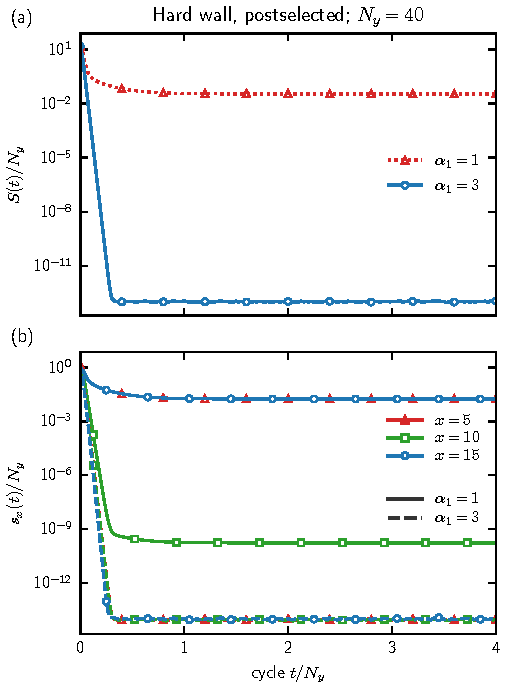
\includegraphics[width=\columnwidth]{postselected_total_spatial_alpha1_alpha3_2x1.pdf}
\caption{Hard-wall postselected purification at $N_x=20$, $N_y=40$,
$\alpha_2=30$, $n_{\rm shell}=1$, and $T=160$ cycles.
Each $\alpha_1=1,3$ run is a single fully postselected trajectory from
a maximally mixed active slab, with raster-$y$ measurements and no feedback.
(a) Total entropy $S(t)/N_y$.
(b) Column entropy $s_x(t)/N_y$, summed over $y$ and the two orbitals,
at $x=5,10,15$. Colors and markers identify columns; solid and dashed
curves identify $\alpha_1=1,3$, respectively.
All 161 cycles are shown with logarithmic entropy and linear rescaled time.
No averaging, fits, or uncertainty bars are applied.
The $\alpha_1=3$ near-zero tails are roundoff-limited.}
\label{fig:postselected-purification-control}
\end{figure}
